\section{System Demonstration}
\label{sec:app_demo}

This section walks through the three primary user flows as they appear in the deployed application.

\subsection{Multimodal Search Flow}

A user opens the application, enters their user ID on the login gate, and is placed in the Active Search tab.
They type the Vietnamese query \textit{``sách về trí tuệ nhân tạo''} (books about artificial intelligence) into the search box and submit.

Internally, the NLLB-200 pipeline detects Vietnamese in under 1\,ms and translates the query to ``books about artificial intelligence''.
The translated query is encoded by BGE-M3, searched against the HNSW text index, and fused with Tantivy BM25 scores via RRF.
While the request is in flight, four animated skeleton placeholder cards occupy the result area.
On response arrival, the placeholders are replaced by result cards showing the cover image, title, author, genre, and score badges: an RRF fusion badge on every card, plus a BGE-M3 badge reflecting text-channel similarity and a CLIP badge reflecting visual-channel similarity where applicable.
Warm-cache end-to-end latency for this step is approximately 59\,ms.

Figure~\ref{fig:search_demo} shows the result page for a representative search query.

\begin{figure}[H]
\centering
\begin{subfigure}{\textwidth}
    \centering
    
\includegraphics[width=0.80\textwidth]{images/chapter6/fig_search_text}
    \caption{Text query: RRF and BGE-M3 badges.}
    \label{fig:search_text}
\end{subfigure}

\vspace{8pt}

\begin{subfigure}{\textwidth}
    \centering
    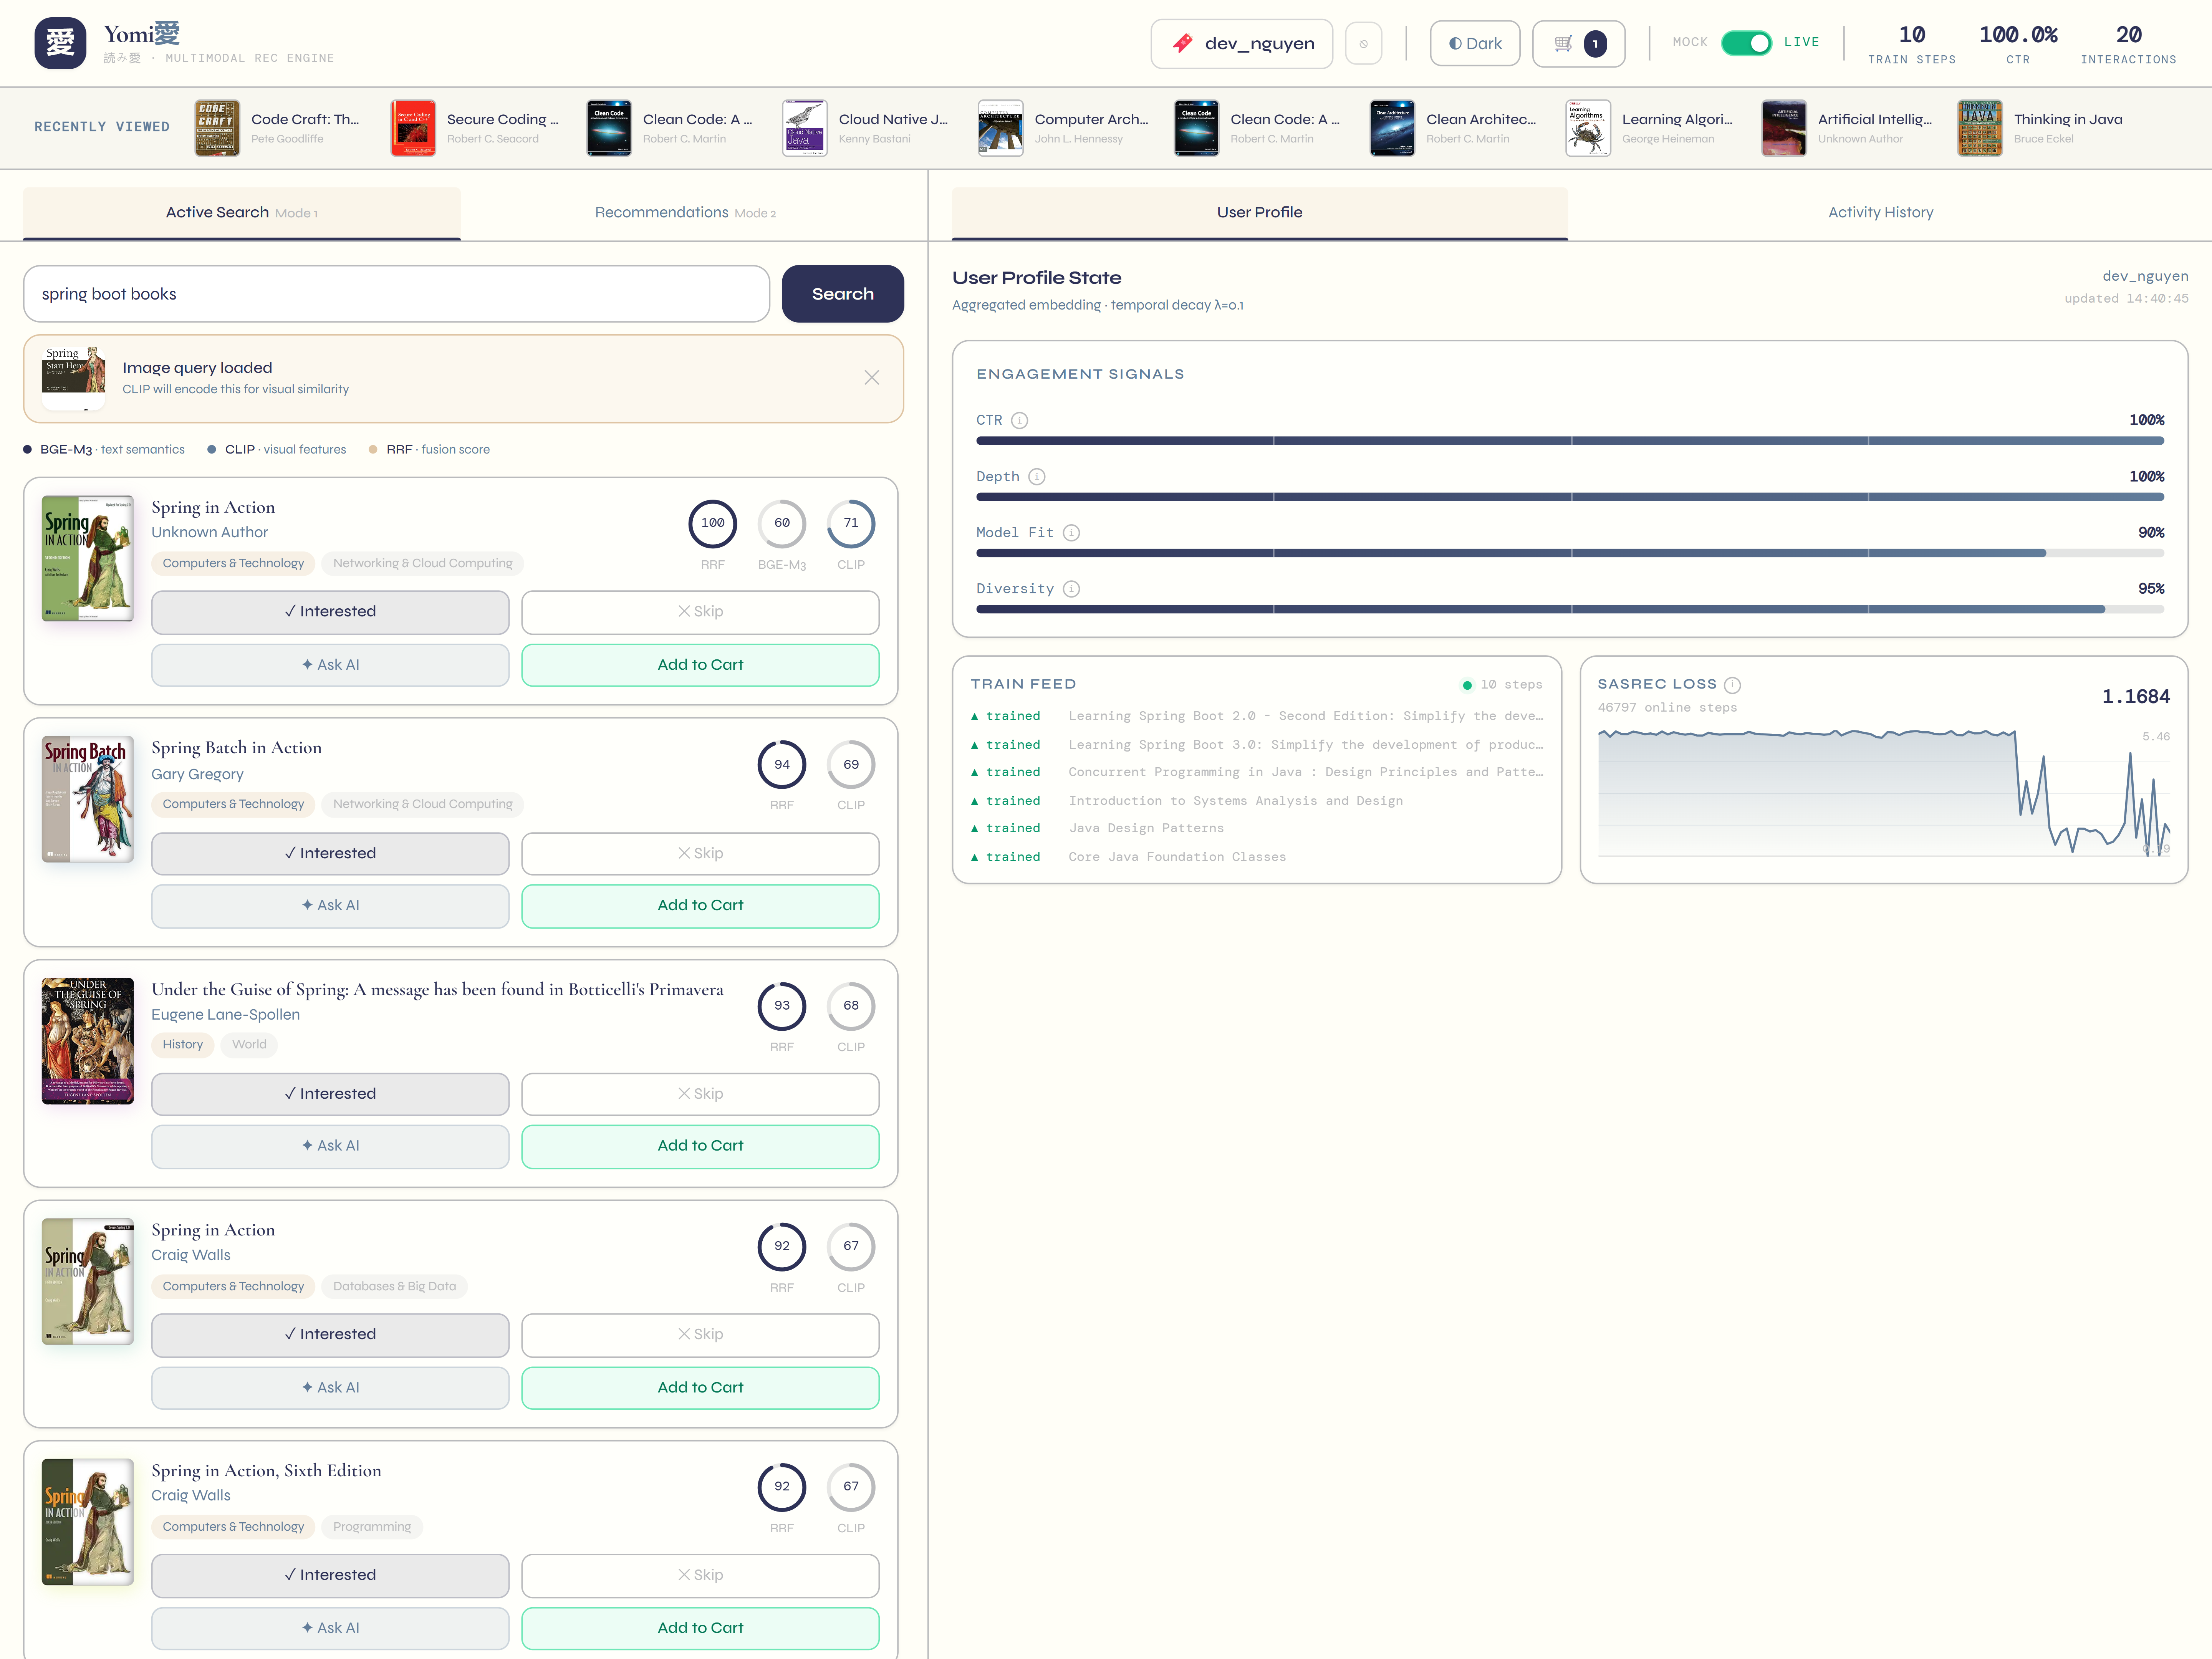
\includegraphics[width=0.80\textwidth]{images/chapter6/fig_search_multimodal}
    \caption{Combined text + image query: RRF, BGE-M3, and CLIP badges.}
    \label{fig:search_multimodal}
\end{subfigure}

\caption{Active Search results (Mode 1). Each result card presents cover image, title, author, genre, score badges, and four interaction controls: \textit{Interested}, \textit{Skip}, \textit{Ask AI} (streaming LLM popover), and \textit{Add to Cart}. (a)~Text-only query shows RRF and BGE-M3 badges. (b)~Combined text and image query additionally shows a CLIP badge, demonstrating the multimodal fusion path.}
\label{fig:search_demo}
\end{figure}

Each result card provides three interaction controls.
Interested logs a click event (reward 1.0), updates the in-memory user profile, and triggers a DIF-SASRec gradient step.
Add to Cart logs a cart event (reward 5.0), appends the item to the in-session cart, and triggers a gradient step.
Ask AI opens an inline streaming popover that calls \texttt{POST /ask\_llm\_stream}; the Qwen2.5 response is rendered progressively under Genre, Plot Summary, and Pitch headings as tokens arrive.

For image queries, the user clicks the camera icon button embedded within the search input to open an upload popover.
A drag-and-drop zone inside the popover accepts cover images; once an image is selected, a thumbnail preview confirms that the CLIP encoder will process it, and the popover can be dismissed.
If both text and image are supplied simultaneously, both encoders run in parallel and their candidate lists are fused by RRF before metadata hydration.

\subsection{Personalised Recommendation Flow}

After a user accumulates at least five interactions, the Recommendations tab (Mode 2) switches from cold-start to personalised mode.
A toast notification confirms the transition to personalised mode.

Figure~\ref{fig:rec_demo} shows the recommendation panel for a warm user.

\begin{figure}[htbp]
\centering
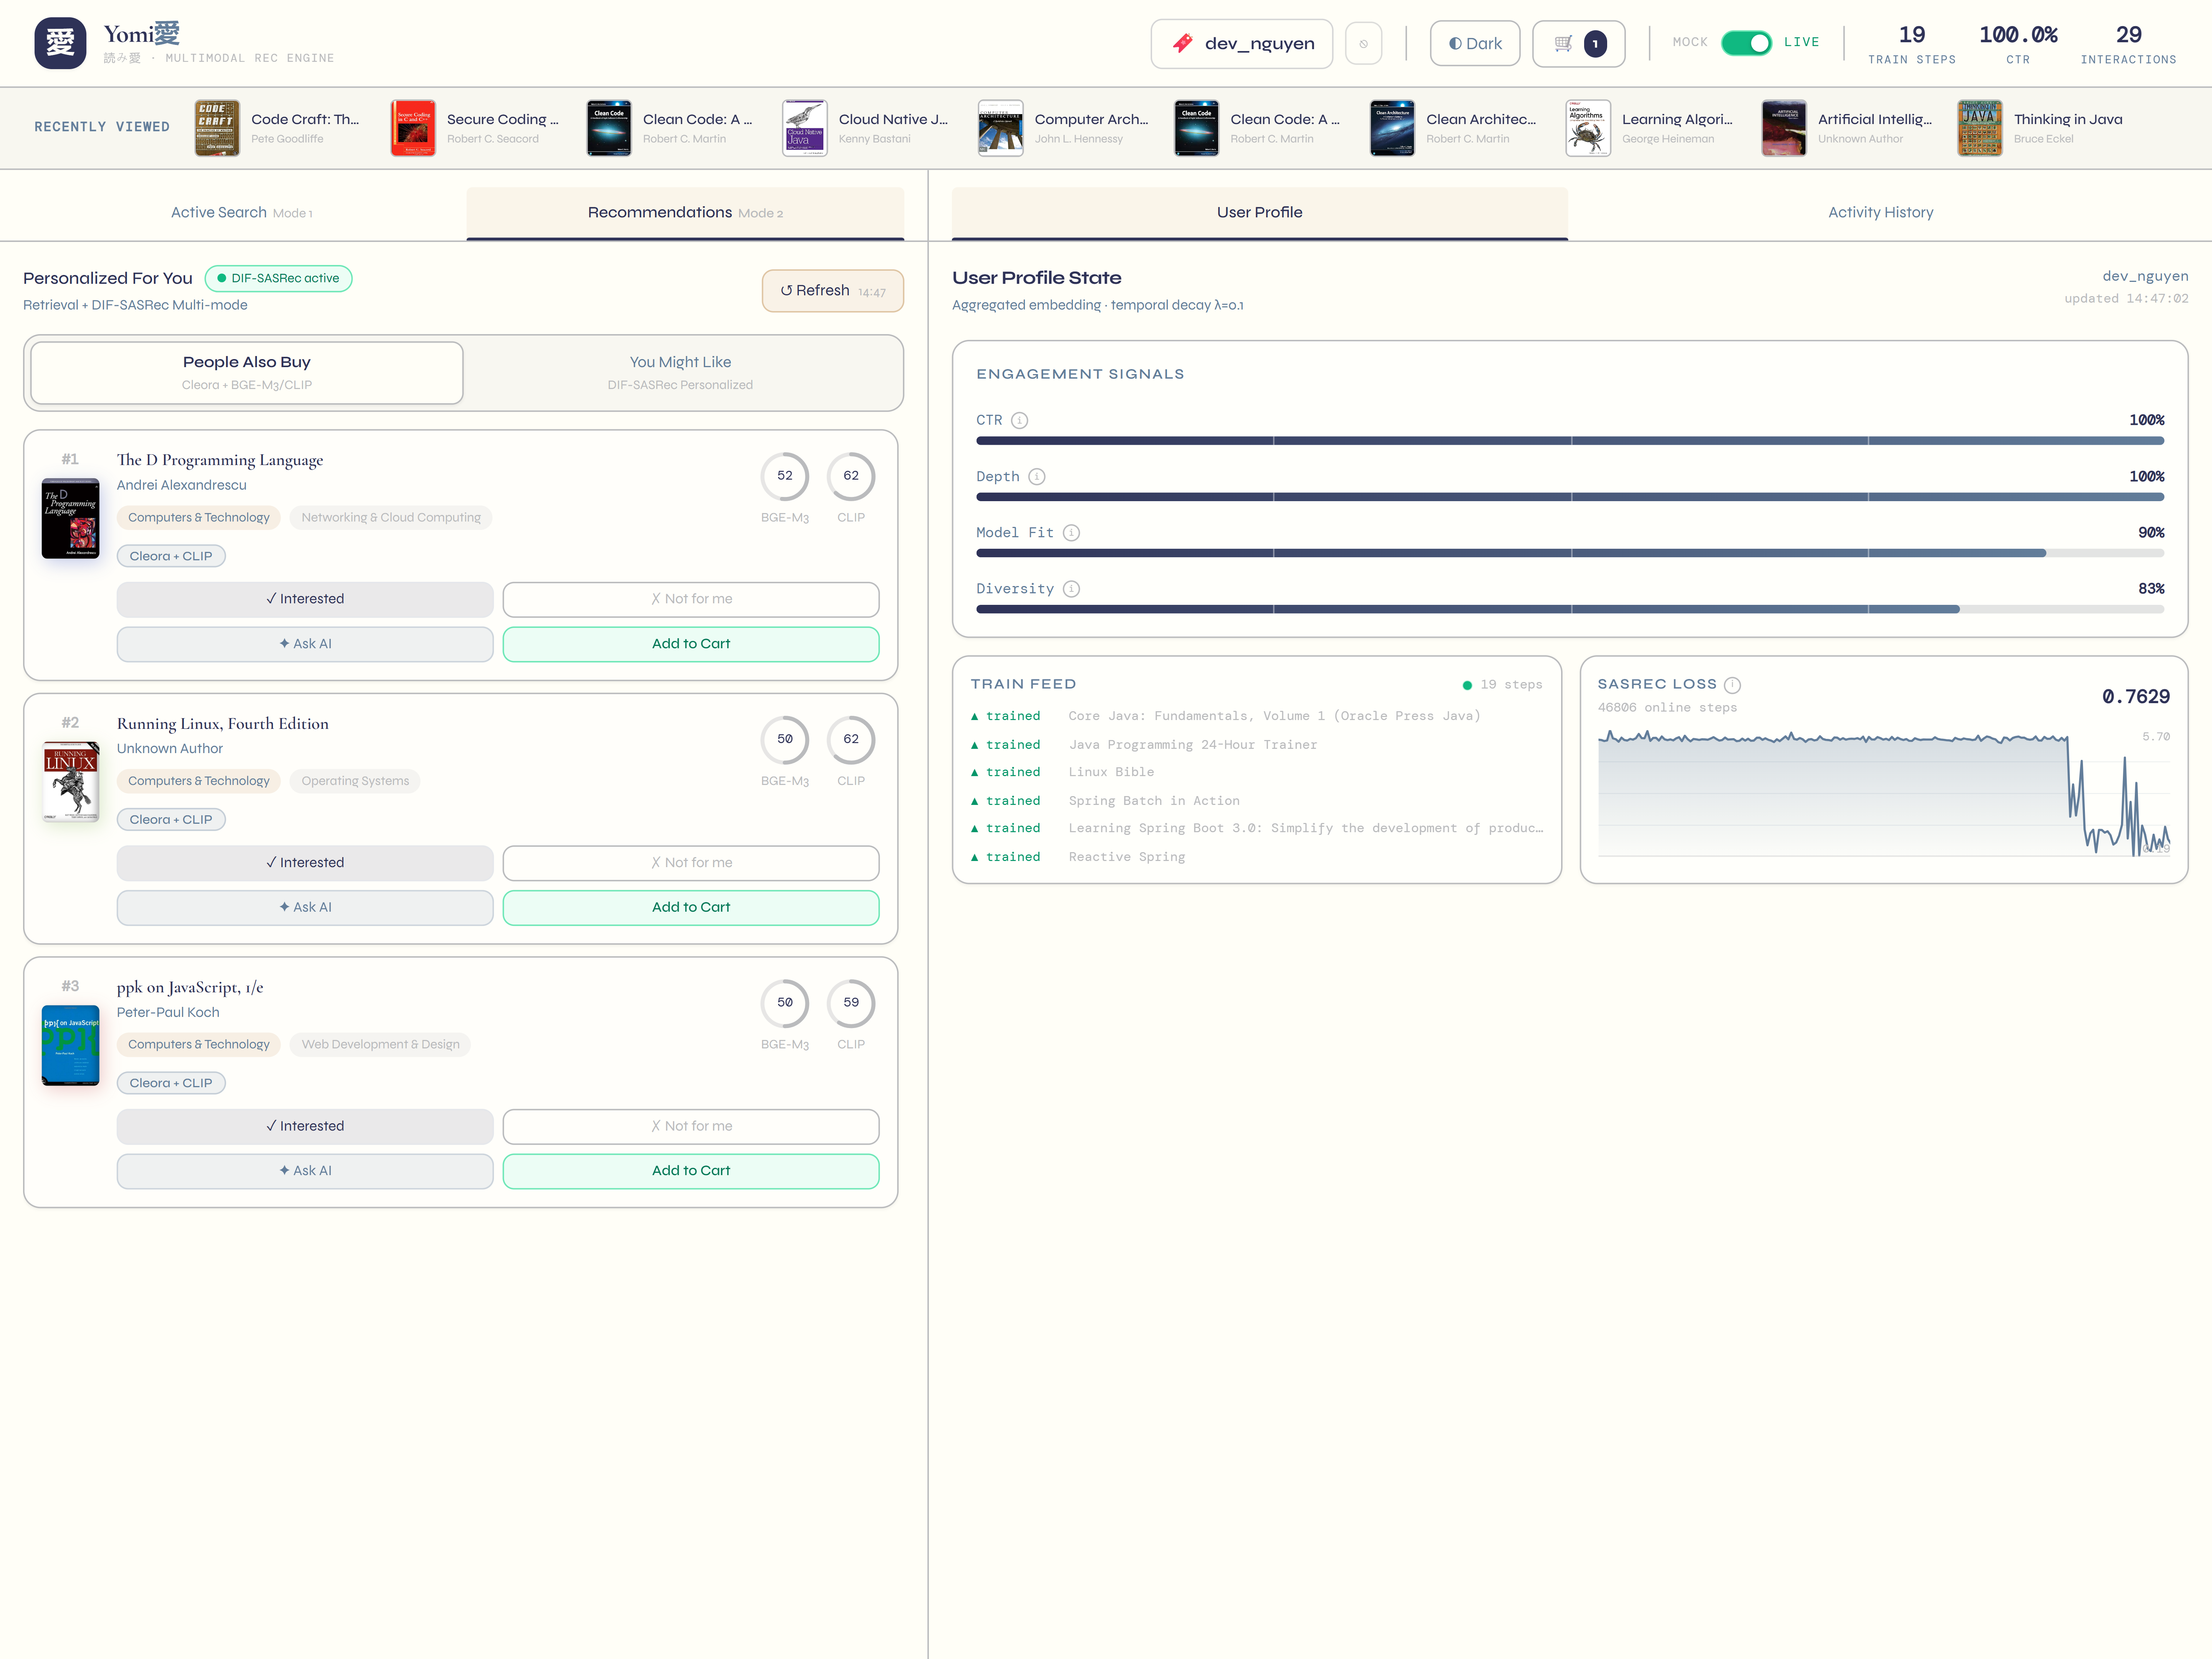
\includegraphics[width=0.92\textwidth]{images/chapter6/fig_rec_pab}
\caption{Personalised Recommendations (Mode 2) for a warm user, displayed as two side-by-side columns.
The People Also Buy column (Pipeline~A) surfaces Cleora co-purchase neighbours re-ranked by the user's BGE-M3 or CLIP profile vector, with cosine-similarity score badges and a \textit{Cleora~+~BGE-M3} or \textit{Cleora~+~CLIP} layer tag on each card.
The You Might Like column (Pipeline~B) applies the DIF-SASRec sequential model, with a SASRec score badge and a \textit{DIF-SASRec} layer tag.
The input-sequence strip above both columns displays the user's most recent click and cart interactions in chronological order, making the model's input visible.}
\label{fig:rec_demo}
\end{figure}

The input-sequence strip is displayed above both recommendation columns when personalised mode is active.
This strip shows the user's most recent click and cart interactions — up to eight items — in chronological order, representing the exact sequence that DIF-SASRec reads when generating the next-item prediction.
The strip makes the sequential model's input visible to the user, providing an explanation for why specific items were recommended.

Recommendations are refreshed automatically every three new interactions.
A manual refresh button forces an immediate reload and displays the last-updated timestamp beside its label.
Items that are new since the previous refresh are highlighted for four seconds.

\subsection{Online Learning Observation}

Every click or cart event triggers a sampled softmax gradient step on the user's personal DIF-SASRec checkpoint.
The SASRec Loss sparkline in the right-side profile panel shows the full loss history as a filled area chart.
A dashed divider marks the boundary between the pretraining phase (checkpoint-loaded, high loss scale) and the online fine-tuning phase (per-user gradient steps, lower scale).
An information tooltip beside the chart title explains the expected scale difference, noting that pretraining uses 512 hard negatives whereas online training samples from the full 3-million-item catalogue, producing a structurally lower loss.
When a gradient step fires, a transient loss-decrease badge is displayed beside the current loss value for 2.5 seconds, confirming that the model has updated.
